\section{Durchführung}
\label{sec:Durchführung}

Die Reservoire der in Abb. \ref{fig:aufbau2} dargestellten Apparatur werden jeweils mit einer Wassermenge von 
$\SI{3}{\liter}$ aufgefüllt. Anschließend werden die Temperaturen $T_1$ und $T_\text{2}$ in den 
Reservoiren, die Drücke $p_\text{a}$ und $p_\text{b}$ im Verdampfungs- bzw. Verflüssigungsbereich und 
die Leistungsaufnahme des Kompressors gemessen. Der Zeittakt beträgt dabei eine Minute. 
Die Messung wird abgebrochen, sobald $T_1$ einen Wert von ca. $\SI{50}{\degreeCelsius}$ 
erreicht hat. 
\begin{figure}
    \centering
    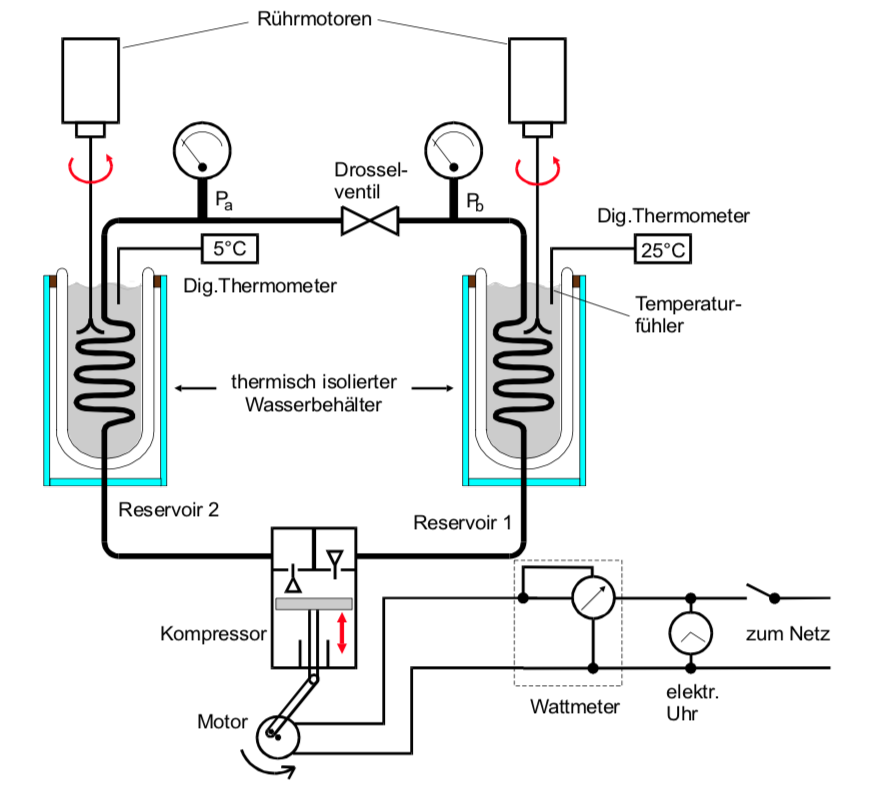
\includegraphics[width=10cm, height=10cm]{build/2.png}
    \caption{Aufbau einer Wärmepumpe sowie der Messapparatur.
    Der Druck $p_b$ und die Temperatur
    $T_1$ beziehen sich auf das Reservoir $\num{1}$. Der Druck $p_a$ und die Temperatur
    $T_2$ beziehen sich auf das Reservoir $\num{2}$.}
    \label{fig:aufbau2}
\end{figure}
